\newpage

% =====================================================================
%====== Table Of contents =============================================
%======================================================================
\tableofcontents
%\listoftodos



\newpage
% =====================================================================
%====== Indledning ====================================================
%======================================================================
\section{Indledning}
Scalextric er en stor producent af elektriske biler, skinner og fjernbetjeninger dertil. Det er populært blandt især børn, at bygge deres egen racerbane og køre om kap. Projektets store udfordring er at modificere en af Scalextrics biler og udstyre dem med sensorer, således at den selv kan køre og justere sin hastighed på en hensigtsmæssig måde.

\subsection{Projektbeskrivelse}
\subsubsection{Problemanalyse}
\label{problemanalyse}
Projektet skal få en elektrisk bil til hurtigst muligt at køre omgange på en vilkårlig bane uden at ryge af banen. For at opnå dette kræves forskellige sensorer, som skal monteres og programmeres. Formålet er at opnå kendskab til programmering i Assembler og opbygning af sensorkredsløb, samt få software og sensorer til at arbejde sammen.  \\
Projektet består af følgende: \\

\begin{itemize}
\item Bluetooth kommunikation med bilen via en given protokol.
\item Byg og montér sensor kredsløb til de forskellige nødvendige sensorer.
\item Algoritme der kortlægger banen.
\item Algoritme der bruger den kortlagt bane og sensor data til at køre med optimal hastighed.
\end{itemize}


\subsubsection{Problemformulering}
\label{problemformulering}
Hvordan opbygges og programmeres en elektrisk bil til selv at kunne køre hurtigste tid på en vilkårlig bane? Denne problemstilling vil vi arbejde med i dette projekt, og dertil skal disse problemer løses: \\

\begin{itemize}
\item Hvordan kommunikeres der med bilen?
\item Hvilke sensorer skal benyttes for at gøre bilen selvkørende med så høj hastighed som muligt?
\item Hvilken elektromagnetisksensor/-aktuator skal bruges?
\item Hvordan detekteres målstregen?
\item Hvordan detekteres sving?
\item Hvordan programmeres microcontrolleren så den kan kortlægge en vilkårlig bane?
\item Hvordan programmeres bilen til at udnytte den kortlagte bane til at køre hurtigst muligt?
\item Hvordan bremser bilen best muligt?
\end{itemize}

\newpage
\subsubsection{Afgrænsning}
I denne opgave begrænser vi os til at bygge sensorkredsløb og programmere microcontrolleren til den elektriske bil. Vi skal ikke bygge bilen fra bunden, men modificere en eksisterende model til at kunne styres gennem vores microcontroller. Bluetooth kommunikationsprotokollen er også bestemt for os, men vi skal selv implementere denne og kan også udvide den. \\

Vores projekt kan derfor fortolkes til at programmere en microcontroller til at modtage signaler fra sensorer og derudfra kortlægge en bane og kontrollere motoren for at opnå den hurtigste omgangstid. 


\subsubsection{Konkurrenceregler}
\label{kon_regler}
Den 29. maj 2015 afholdes Pole Position konkurrencen. Her vinder det hold, som har den hurtigste omgangstid. Der er visse krav til bilen for at gøre konkurrencen fair. Bilen skal kunne køre af sig selv og skal således starte når den sættes på banen. Det skal dog være muligt at sætte en hastighed eller stoppe bilen vha. Bluetooth. Denne kommunikation skal overholde en protokol, som senere vil blive uddybet. Selve banen består kun af rene højre eller venstre sving, dvs. at der minimum vil være en lige skinne mellem to sving. Bilens karosseri, dæk og undervogn må ikke ændres. Det er dog tilladt at lave mindre ændringer for at gøre plads til sensorer og lignende. Der må ikke monteres permamagneter på bilen. Magneten som er monteret på bilen fra fabrikken må dog blive siddende. Der skal anvendes en elektromagnetisk sensor og/eller -aktuator i projektet. Dette kan f.eks. være i form af en elektromagnet. 


\subsection{Rapportstruktur}
Projektet består af flere dele, hvor microcontrolleren er i centrum. Delene har forskellige realationer til microcontrolleren som \ref{Strategi} illustrerer.\\

\begin{figure}[h!]
\center
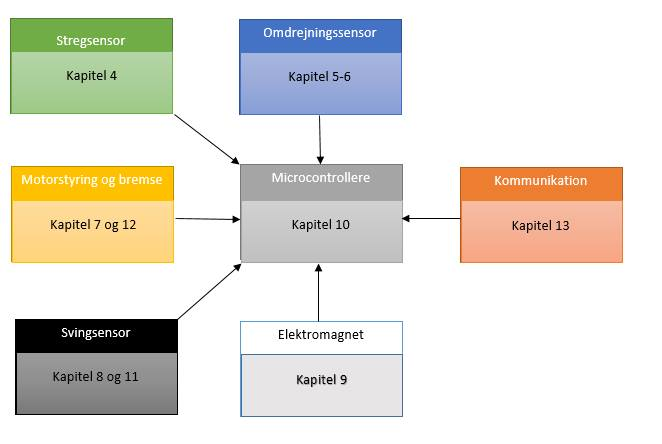
\includegraphics[scale=0.4]{./Graphics/Strategi}
\caption{Overblik over hovedemner, dvs. strategi}
\label{Strategi}
\end{figure}

Microntrolleren styre forsyningen til motoren. Omdrejningssensor tæller motorens omdrejninger og sender informationer tilbage til microcontrolleren. Svingsensor sender informationer om til processoren om sving. Stregsensoren detektere startlinjen og informere controlleren om dette. Microcontrolleren styrer forsyningen til elektromagneten. Derudover er der en tovejs kommunikation mellem bluetooth-modulet og microcontrolleren. \\
Udover at blokkene til sammen beskriver produktet, giver dette også en oversigt over rapportens opbygning. De enkelte dele udgør hovedafsnittene i rapporten. Vha. dette kort kan læseren nemt navigere rundt i rapporten uden at miste overblik. 